\chapter{Progettazione}
\label{ch:progettazione}

Il seguente lavoro di tesi riguarda l'impiego di tecniche innovative nel campo dell'IoT, nello specifico, la progettazione e la valutazione di reti di monitoraggio mesh indoor basate sul nuovo standard fornito da Bluetooth SIG, la tecnologia \texttt{Bluetooth Mesh}.
A tale standard è stato accostato come tecnologia di supporto uno standard ampiamente diffuso nel mondo della comunicazione, ovvero lo standard \textit{\texttt{IEEE 802.11}}. L'impiego sul medesimo nodo di entrambe le tecnologie garantisce sia la comunicazione con i nodi in grado di supportare solo uno dei due standard sia la possibilità di scegliere la tecnologia da utilizzare in base al carico di lavoro e alle situazioni dell'ambiente circostante.\\

\noindent L'obiettivo preposto ha come scopo quello di garantire la comunicazione tra dispositivi IoT in un ambiente indoor (in qualsiasi situazione), cercando di massimizzare le prestazioni della rete e allo stesso tempo controllare e ove possibile minimizzare i consumi energetici. La scelta è ricaduta sulle due tecnologie preannunciate, poiché al giorno d'oggi esse risultano presenti in qualsiasi tipologia di apparato d'uso quotidiano.\\
Al fine di salvaguardare i consumi energetici la tecnologia prevalentemente utilizzata come mezzo di comunicazione risulta Bluetooth Mesh. L'impiego di tale tecnologia comporta un dispendio energetico, in fase di trasmissione, inferiore rispetto al Wi-Fi. A tal proposito, è maggiormente soggetta alle interferenze dell'ambiente circostante, il che potrebbe compromettere le prestazioni della rete causando la perdita di pacchetti.\\
% ALGORITMO
Per fronteggiare questa situazione è stato implementato un algoritmo dinamico in grado di determinare, in tempo reale, quando un pacchetto risulterà perso e solo in tale circostanza provvederà ad inviarlo nuovamente, questa volta tramite la tecnologia di supporto.
Ogni pacchetto, contrassegnato tramite un identificativo, verrà inviato attraverso la tecnologia Bluetooth e verrà giudicato come perso solo nel momento in cui il tempo trascorso dall'invio risulterà superiore a quello indicato da una soglia, aggiornata costantemente, alla ricezione di un pacchetto Bluetooth.
Nell'aggiornare il valore di soglia, che determina la perdita di un pacchetto, si terrà in considerazione anche degli eventuali ritardi che potrebbero insorgere dato che il carico di lavoro, della rete, piuttosto elevato. Così facendo, si cercherà di evitare un giudizio affrettato sullo `stato' di un pacchetto, evitando ritrasmissioni inutili che provocheranno solo operazioni infruttuose alla rete, dato che quel pacchetto avrà subito solo un ritardo lievemente più alto rispetto alla media determinata osservando i pacchetti in transito in quell'istante e quindi non risulterà perso. Allo stesso tempo si cercherà di minimizzare il più possibile i ritardi relativi alla ritrasmissione di un pacchetto giudicato come ``perso''. Questo comportamento sarà possibile solo analizzando continuamente lo stato della rete e variando la soglia in base alle sensazioni percepite.

\begin{figure}[!ht]
    \centering
    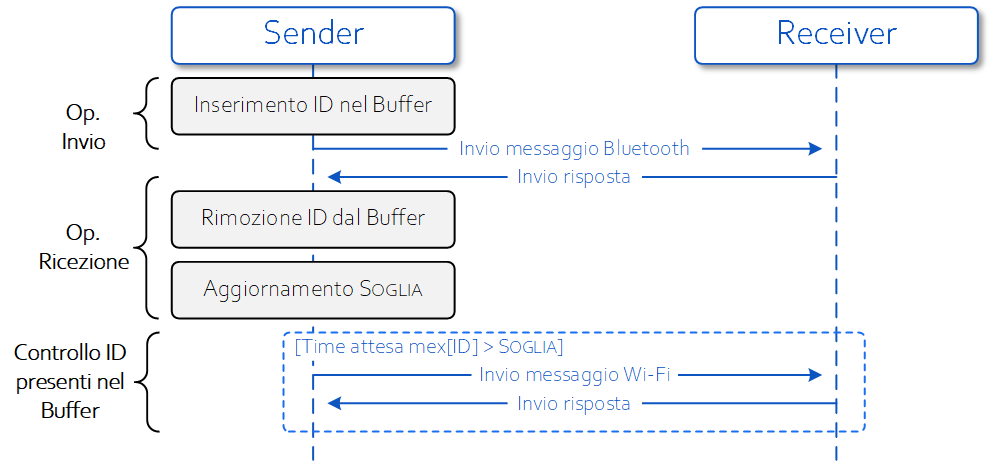
\includegraphics[width = \textwidth]{images/algoritmo_sequence.png}
    \caption{Sequence Diagram - Algoritmo Dinamico}
    \label{fig:sequence_algorithm}
\end{figure}

\noindent Osservando la figura \ref{fig:sequence_algorithm} relativa al comportamento dell'algoritmo dinamico è possibile individuare un'operazione d'invio che prevede appunto l'invio di un messaggio tramite la tecnologia Bluetooth, dopo avere memorizzato l'identificativo corrispondente all'interno di un Buffer. Questa operazione verrà eseguita con una frequenza definita in base al testbed da eseguire. \\
In seguito, qualora il messaggio non risulterà perso, si verificherà un'operazione di ricezione, la quale verrà innescata, dal ricevimento di una risposta. A seguito seguiranno le operazioni che consentiranno la rimozione dell'identificativo corrispondente dal Buffer e l'aggiornamento del valore di soglia.\\
Con la medesima frequenza con cui viene effettuata l'operazione d'invio, verrà eseguita anche l'operazione di check degli identificativi presenti all'interno del Buffer. Qualora il tempo d'attesa di un identificativo risulterà maggiore del valore di soglia, allora si procederà con l'invio impiegando la tecnologia Wi-Fi.\\

\noindent Una volta implementato il codice che consentirà di operare come preannunciato si passerà alla fase di valutazione del modello realizzato. La valutazione in merito al comportamento della rete riguarderà sia il variare della distanza tra mittente e destinatario sia il variare del carico di lavoro. Con `carico di lavoro', si intende la frequenza con cui vengono immessi i messaggi nella rete e ai fini della valutazione è molto importante il metodo di comunicazione request-response. Utilizzando tale paradigma, un messaggio viene definito come perso, solo nel momento in cui non sopraggiunge al Client la risposta da parte del Server.

%%%%% L'obiettivo principale prevede l'utilizzo della tecnologia BLE poiché comporta meno dispendio d'energia in trasmissione e nel momento in cui la rete risulta essere piuttosto carica di lavoro si potrebbe verificare la perdita di alcuni pacchetti durante la comunicazione. L'algoritmo realizzato consente di stabilire, in tempo reale, quando un pacchetto risulta perso e solo in tale circostanza inviarlo tramite la tecnologia di supporto. Con tale algoritmo si è cercato di evitare duplici invii e quindi giudicare troppo frettolosamente lo stato di un pacchetto e allo stesso tempo minimizzare il più possibile i ritardi relativi alla ritrasmissione di un pacchetto giudicato perso. La soglia che consente di definire come ``perso'' un pacchetto risulta essere dinamica, varia in base alla condizioni della rete.

\begin{figure}[!ht]
    \centering
    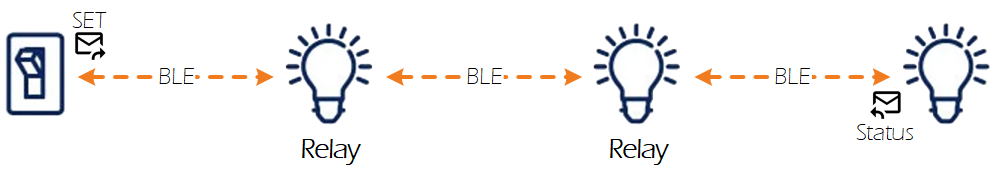
\includegraphics[width = \textwidth]{images/Mesh_network_2.png}
    \caption{rete Bluetooth Mesh}
    \label{fig:mesh_network}
\end{figure}

\noindent Come descritto nella sezione \textit{\nameref{subsub:messaggi}} (\ref{subsub:messaggi}), la comunicazione tra i nodi della rete può avvenire tramite diverse tipologie di messaggi. Tra le tipologie supportate si è pensato di impiegare messaggi di tipo \texttt{SET}, in grado non solo di modificare lo stato di un elemento e quindi rendere percepibile all'utente la ricezione e la gestione di un messaggio, ma anche in grado supportare il meccanismo di acknowledgment e quindi garantire un feedback anche al dispositivo mittente. Quindi alla ricezione di un messaggio ad esso destinato, il nodo provvederà ad attuare il cambio di stato comunicato e successivamente procederà all'invio di un feedback (conferma di ricezione) al mittente. Per quest'ultimo messaggio, lo standard prevede una tipologia appropriata, ovvero un messaggio di tipo \texttt{STATUS}, il quale contiene lo stato assunto dall'elemento interessato.\\

\noindent Con l'impiego di questa modalità di comunicazione, garantita direttamente dallo standard Bluetooth Mesh, si riesce a soddisfare il criterio di comunicazione bidirezionale, ma analizzando ulteriormente le specifiche definite dallo standard in termini di gestione dei messaggi ci ha portato a supporre l'eventualità del sorgere di alcune problematiche legate alla modalità di comunicazione che avremmo voluto ottenere. \\ % Invio di un mex alla stessa destinazione solo dopo aver atteso la scadenza del timer o la ricezione del ack 
La tipologia di messaggi (con acknowledgment) prevede la configurazione di un parametro ``timeout'' al fine di determinare l'evento di perdita e procedere con una ritrasmissione del messaggio. Questo stratagemma, fornito direttamente dallo standard, fa sì che finché non viene innescato tale evento o non viene ricevuta la conferma di ricezione, il sistema impedisce l'invio di ulteriori messaggi alla medesima destinazione. Solo al verificarsi di una delle due condizioni è possibile inviare un nuovo messaggio a tale indirizzo. \\
Ai fini di questo lavoro la suddetta situazione risulta essere troppo stringente, allora si è provveduto ad implementare un meccanismo specifico evitando di utilizzare il meccanismo di acknowledgment fornito dallo standard.\\ 
Il meccanismo proposto prevede lato mittente l'utilizzo di semplici messaggi sempre di tipo \texttt{SET}, ma questa volta senza acknowledgment. L'impiego di un messaggio di tipo \texttt{SET} consente di innescare un cambiamento di stato nel dispositivo destinatario, il quale invece, dovrà supportare un meccanismo di risposta personalizzato al fine di garantire l'avvenuta ricezione di un determinato messaggio. Il destinatario, alla ricezione di un determinato messaggio, dovrà elaborarlo e individuare l'elemento e lo stato da attuare, dopodiché procedere con la creazione di un messaggio di risposta (di tipo \texttt{STATUS}) contenente lo stato assunto. Dopo aver eseguito tutte queste operazioni potrà spedire il messaggio al client e procedere con l'attuazione del cambiamento di stato comunicato.\\ % Failed to send Generic Set message --- Busy sending message to DST

\noindent Per costruire una rete così come mostrato in figura \ref{fig:mesh_network} è necessario introdurre dei dispositivi intermedi al fine di garantire, al messaggio, il raggiungimento del destinatario. Tali dispositivi avranno il compito di inoltrare all'interno della rete tutti quei messaggi non destinati ad essi, rispettando le specifiche relative alla feature ``relay'' messa a disposizione da Bluetooth Mesh (\textit{\nameref{subsub:features}}) ed eseguendo il meccanismo di flooding dei dati descritto nella sezione \textit{\nameref{subsub:managed_flooding}}. Una volta implementata tale rete, nel rispetto delle specifiche descritte in precedenza,
si procederà alla valutazione delle prestazioni eseguendo dei testbed. La predetta configurazione prevederà esclusivamente l'impiego della sola tecnologia Bluetooth Mesh.\\
Poiché l'impiego di questa tecnologia risulta molto soggetta alle interferenze e alle condizioni dell'ambiente circostante si è pensato ad una riduzione sostanziale delle prestazioni nel momento in cui il carico di lavoro risulterà oneroso, con conseguenza congestione della rete, la quale comporterà una perdita di pacchetti ed un aumento della latenza.\\
Per fronteggiare una tale situazione e quindi garantire delle prestazioni elevate della rete anche con un carico di lavoro oneroso si è pensato di accostare un'altra tecnologia, al fine di ripartire il lavoro tra le due tecnologie, portando ad avere ottime prestazioni in qualsiasi circostanza. La scelta della tecnologia di supporto è ricaduta su \texttt{IEEE 802.11}, poiché ampiamente presente in qualsiasi tipologia di apparato di quotidiano utilizzo.\\
Inizialmente, si è pensato di adottare l'approccio Wi-Fi Mesh, in modo da avere la medesima infrastruttura di rete per entrambe le tecnologie. Con la possibilità di interconnettere i nodi, distribuiti su una vasta area fisica, sotto un'unica WLAN (Wireless Local-Area Network), in cui non si ha un singolo nodo centrale, denominato Acess Point, direttamente collegato a tutti gli altri nodi, bensì ai singoli nodi è consentito connettersi con i nodi vicini, i quali si assumono la responsabilità reciproca di divulgare la comunicazione all'interno della rete.\\
A seguito di opportune osservazioni è stato individuato, che adoperare sul medesimo nodo sia la tecnologia Bluetooth Mesh sia la tecnologia Wi-Fi Mesh risultava infattibile per la quantità di memoria richiesta per il loro funzionamento. Difatti, il modus operandi legato a tali tecniche prevede una quantità di memoria nettamente maggiore di quella di cui risultano dotati dei semplici dispositivi a nostra disposizione (\texttt{ESP32}). \\
Analizzando anche l'area di copertura dei dispositivi, in cui il raggio di trasmissione garantito dalla tecnologia Bluetooth è nettamente inferiore rispetto a quello Wi-Fi, ci è sembrato alquanto oneroso e poco produttivo l'impiego di un tale approccio, poiché tale area sarebbe stata coperta anche impiegando una rete Wi-Fi tradizionale.\\
Quindi, per la tecnologia di supporto si è ricorso all'utilizzo di una rete Wi-Fi tradizionale, la quale ci avrebbe garantito la possibilità di comunicare con tutti gli apparati che andranno a costituire la rete in un contesto indoor e non avremmo avuto problemi, in termini di memoria, in fase d'esecuzione. Tale approccio prevederà l'introduzione di un'entità esterna avente la funzione di Access Point (\texttt{AP}) a cui saranno direttamente connessi tutti gli altri nodi della rete e a cui spetterà il compito di inoltrare il pacchetto al nodo destinatario.

\begin{figure}[!ht]
    \centering
    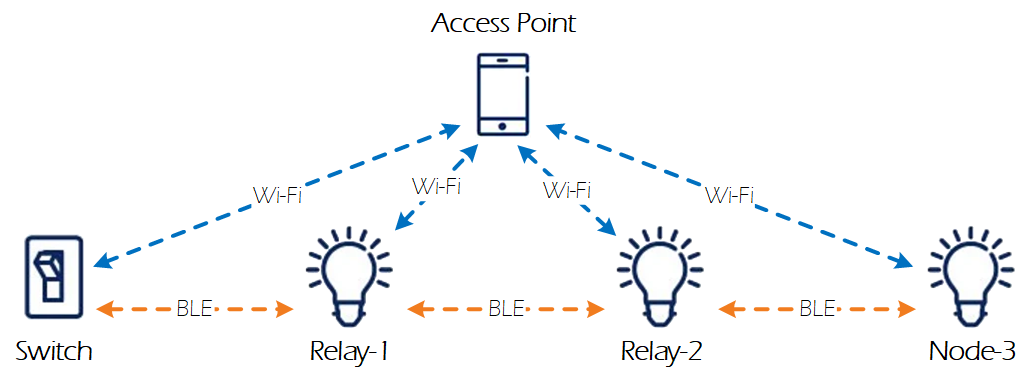
\includegraphics[width = \textwidth]{images/BLE_WiFi_2.png}
    \caption{rete Bluetooth Mesh - Wi-Fi}
    \label{fig:mesh_network_wifi}
\end{figure}

% La suddetta tecnologia, però, prevede un dispendio d'energia maggiore per la trasmissione di un pacchetto e in base a ciò si è presupposto che il raggio di copertura garantito da quest'ultima risultasse nettamente maggiore rispetto a quello del BLE, quindi impiegando un solo access point si potrà comunque garantire la comunicazione tra tutti gli apparati che andranno a costituire la rete in un contesto indoor.

\noindent Definite le tecnologie da impiegare nel seguente lavoro è stato necessario determinare come farle interagire tra loro al fine di diminuire la perdita di pacchetti, minimizzare i ritardi in fase di ritrasmissione e cercare di salvaguardare i consumi energetici.\\
Per fronteggiare tale situazione si è pensato di utilizzare come tecnologia preferita, lo standard Bluetooth Mesh e nel momento in cui si identifica la perdita di un pacchetto provvedere alla ritrasmissione utilizzando la tecnologia di supporto (più dispendiosa dal punto di vista energetico). In tal modo, con l'alternanza delle due tecnologie si allevia il carico di lavoro sulla tecnologia principale e allo stesso tempo si cerca di mantenere alte le performance delle rete.\\

\noindent Osservando la figura \ref{fig:sequence_algorithm_2} possiamo individuare le due fasi che costituiscono l'algoritmo descritto in precedenza. Tale algoritmo, inizialmente si troverà in uno stato di sleep, nel quale sarà possibile inviare solo messaggi attraverso la tecnologia Bluetooth, il che consentirà alla rete di giungere a pieno regime. Una volta giunto in tale stato si passerà ad una modalità attiva in cui si procederà sempre all'invio dei messaggi impiegando un tasso trasmissivo determinato dal testbed da eseguire. Nel mentre si eseguirà l'operazione di invio tramite Bluetooth, verrà analizzato lo stato della rete e ogni qualvolta verrà innescato l'evento di ricezione si procederà con l'operazione di ricezione (mostrata nel grafico \ref{fig:sequence_algorithm}) che comprenderà anche l'aggiornamento della soglia. Contemporaneamente, verrà eseguito anche il controllo sugli identificativi per verificare se ci sono pacchetti definiti ``persi''. Nel caso l'esito di tale controllo risulterà positivo, allora si procederà con l'invio del pacchetto tramite il Wi-Fi.

\begin{figure}[!ht]
    \centering
    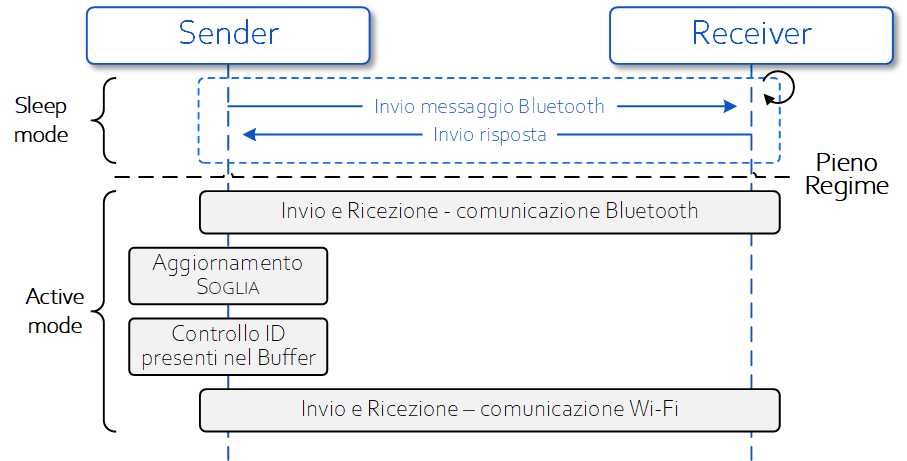
\includegraphics[width = 0.99\textwidth]{images/algoritmo_sequence_2.png}
    \caption{Sequence Diagram - Algoritmo Dinamico}
    \label{fig:sequence_algorithm_2}
\end{figure}

\noindent La realizzazione di una tale soluzione è stata pensata avvalendosi di un buffer contenente l'identificativo del messaggio da inviare. All'atto dell'invio di un messaggio tramite Bluetooth, l'identificativo corrispondente verrà inserito nel buffer e verrà rimosso solo nel momento in cui avverrà la ricezione del corrispondente messaggio di risposta, altrimenti, trascorso un intervallo di tempo, definito dal valore di soglia, verrà trasmesso un nuovo messaggio contenente il medesimo identificativo, questa volta però, utilizzando la tecnologia Wi-Fi (soluzione mostrata in figura \ref{fig:sequence_algorithm}. 
Operando in questo modo si tenterà di decongestionare la trasmissione Bluetooth, utilizzata per la gestione di gran parte dei messaggi.  

\begin{figure}[!ht]
    \centering
    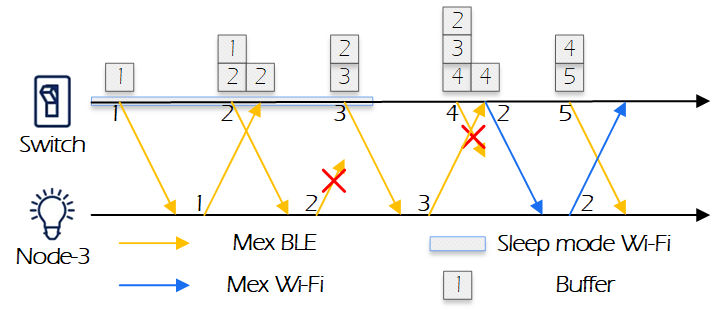
\includegraphics[width = \textwidth]{images/Algoritmo_dinamico.png}
    \caption{Algoritmo dinamico per utilizzare la tecnologia BLE Mesh e Wi-Fi}
    \label{fig:algoritmo dinamico}
\end{figure}

\noindent Così come accaduto con la prima soluzione, anche quest'ultima dovrà essere valutata. Quindi, implementati tutti i nodi, affinché si potessero usare entrambe le tecnologie, si è passati alla definizione dei casi di test.\\
L'idea a monte è quella di definire un intervallo di tempo, ovvero la durata del test e andare a modificare la frequenza con cui i messaggi vengono immessi nella rete, in modo da comprendere il suo comportamento nelle varie situazioni. 
Un'altra idea prevede di variare la distanza tra il nodo mittente e il destinatario e allo stesso tempo l'introduzione di nodi intermedi, facendo sì che ogni messaggio inviato passasse attraverso tali nodi prima di giungere a destinazione.\\
Una volta stabiliti i test è sorto il dilemma di come comunicare il test da eseguire. Ovvero come configurare un nodo affinché venisse eseguito un determinato test, anche perché le configurazione e i parametri risultavano essere diversi.\\
Una soluzione molto semplice, ma piuttosto dispendiosa, sarebbe stata quella di modificare i parametri del test direttamente mettendo mano all'interno dal codice. Lo svantaggio di tale soluzione riguardava il tempo impiegato, ogni qualvolta si cambiasse test, per modificare i parametri e successivamente reinstallare il codice sulla board. Per evitare tutte queste operazioni, si è pensato ad una soluzione un po' più complessa da gestire inizialmente, che però una volta definita, consentisse di comunicare qualsiasi configurazione al nodo senza dover caricare ogni volta il codice sulla board. Anche se tale processo coinvolgerà solo il nodo avente l'incarico di immettere i messaggi nella rete.\\
Così facendo il nodo potrà ricevere la configurazione e comportarsi di conseguenza. La soluzione prevede l'impiego di una comunicazione seriale, attraverso la quale sarà possibile indicare mediante una regola i parametri necessari al fine di configurare il nodo, avviare la simulazione ed ottenere in output il log di tale test.\\
L'operazione di configurazione riguarderà un solo nodo all'interno della rete, identificato con il nome di client, il quale avrà l'incarico di immettere i messaggi per gestire i vari elementi di cui essa risulta essere composta. Tale nodo può essere visto come un telecomando in grado di gestire l'accensione e lo spegnimento ma, anche la gestione della luminosità di un qualunque altro dispositivo inglobato nella rete, come potrebbero esserlo delle luci presenti all'interno di un contesto abitativo.\\
Cercando la soluzione efficace per affrontare questa problematica emersa, si è pensato all'impiego di un dispositivo \texttt{UART}\footnote{\textit{Universal Asynchronous Receiver-Transmitter}, un dispositivo hardware utilizzato per far dialogare tramite porta seriale un dispositivo di input/output con il nodo client}.

\begin{figure}[!ht]
    \centering
    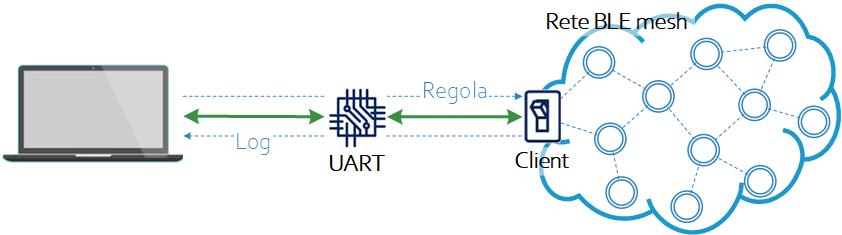
\includegraphics[width = \textwidth]{images/Uart.png}
    \caption{Architettura Rete BLE mesh - Test}
    \label{fig:mesh_network_uart}
\end{figure}

\noindent L'impiego di semplici dispositivi dotati di non molta memoria (tra l'altro sfruttata al massimo per poter eseguire i due stack protocollari) ha fatto sì che la creazione di un file di log, necessario per poter eseguire future analisi sull'operato, avvenisse non sul nodo ma su un dispositivo esterno. Anche in tale circostanza ci è venuto in soccorso il dispositivo \texttt{UART}. Poiché esso consente una comunicazione bidirezionale, potrà essere sfruttato anche per comunicare il verificarsi di ogni singolo evento di nostro interesse.\\

\noindent Per poter passare all'esecuzione dei testbed e vedere all'opera quanto è stato realizzato è fondamentale, come previsto dallo standard, un processo di provisioning al fine di consentire la creazione della nostra rete. In base a quanto detto nel capitolo \ref{ch:Ble_mesh}, il procedimento di provisioning prevede l'impiego di un dispositivo avente il ruolo di provisioner (sezione \ref{sec:provisioning}).
A tal proposito verrà adoperando uno smartphone con su installata un'apposita applicazione che consentirà la creazione, la configurazione e la gestione della rete mesh. Una volta creata la rete e configurati tutti i nodi sarà possibile procedere con l'esecuzione dei test utilizzando i parametri di configurazione ricevuti appositamente tramite seriale.\\
Con l'impiego di entrambe le tecnologie, il dispositivo una volta entrato a far parte della rete mesh non avrà concluso la fase di configurazione, ma dovrà procedere con la sottoscrizione ad una determinata rete Wi-Fi, utilizzata solo per trasmettere i messaggi (denominati come `persi' con la tecnologia BLE mesh) tra i nodi della rete. \\
Solo dopo aver inizializzato e configurato entrambe le tecnologie, la fase di configurazione risulterà terminata e sarà possibile procedere con la fase di test vera e propria.\\

\noindent Gli eventi generati durante l'esecuzione del test verranno memorizzati attraverso un file di log e in secondo luogo, verranno analizzati ed infine confrontati i risultati ottenuti dall'esecuzione delle due soluzioni descritte in questo capitolo.\\
